\section{Baseline Methods}
\label{sec:method}
In this section, we present baseline methods for 
the two proposed tasks. 

\subsection{Object Co-location Classification}
\label{sec:classify} 
%\textbf{Problem Statement} 
Given a sentence $s$ mentioning a pair of physical objects 
\textless$e_i,e_j$\textgreater, 
we denote such a triple as an \textit{instance} \textless$s,e_i,e_j$\textgreater~. 
We formulate the first task as a binary classification problem, which aims to determine whether or not $e_i$ and $e_j$ are physically located near each other 
in a scene, depicted in the sentence $s$.
For example, suppose $e_i$ is ``dog" and $e_j$ is ``cat'', $s_1$ = ``\textit{The King puts his dog and cat on the table.}'', 
and $s_2$ = ``\textit{My dog is older than her cat.}''.
Then the answer to the instance \textless$s_1,e_i,e_j$\textgreater ~is \textit{True}, 
since $s_1$ is describing a scene in which both the dog and the cat are present
and are near each other.
On the other hand, the dog and the cat in $s_2$ do not have to be 
located near since $s_2$ is talking about a general comparison, 
therefore the answer to  the instance \textless$s_2,e_i,e_j$\textgreater~
is \textit{False}
We propose two baseline methods in the two following sections, 
a feature-based method and an LSTM-based method.

\subsubsection{Feature-based Methods}
We propose several of features to be extracted from 
a sentence containing the mentions of at least physical objects:

\noindent
\textit{Bag of Words} (BW)
This is a set of words that ever appeared in
the sentence. Each dimension in this feature represents the occurrences of each word in the vocabulary. (number of features equals to vocabulary size)

\noindent
\textit{Bag of Path Words} (BPW)
This is the set of words that appeared on
the shortest dependency path between objects $e_i$ and $e_j$ in the dependency parse
tree of the sentence, plus the words in the two subtrees rooted at $e_i$ and
$e_j$ in the parse tree. These words are believed to be more important
than the rest in our task. (number of features equals to vocabulary size)

\noindent
\textit{Bag of Adverbs and Prepositions} (BAP)
We collect a list of 244 adverbs\footnote{\url{https://www.espressoenglish.net/100-common-english-adverbs/}} and prepositions\footnote{Obtained from ``Single words'' and ``Two words'' list on \url{https://en.wikipedia.org/wiki/List_of_English_prepositions}}, 
and use their existence in the sentence as binary features. (244 features)

\noindent
\textit{Global Features} (GF)
The length of the sentence, the number of nouns, verbs, adverbs, adjectives, determiners, prepositions and punctuations in the whole sentence. (8 features)

\noindent
\textit{Shortest Dependency Path Features} (SDP)
From the dependency parse
tree of the sentence and the shortest path between the two objects 
$e_i$ and $e_j$, we capture the same above features in this path. (8 features)

\noindent
\textit{Semantic Similarity Features} (SS)
We compute the cosine similarity between the word vectors of the two objects using word embeddings from pre-trained glove vectors and our corpus respectively. (2 features)

Obtaining such features for every instances, 
we then feed them into a Support Vector Machine (SVM) classifier. 
For hyperparameters selection and tuning, please refer 
to experiments. 

\subsubsection{LSTM-based Methods}
Although above features are both informative and easy to implement, 
they involve little sequential information such as the word order.
Recurrent Neural Networks (RNNs), 
especially Long Short-Term Memories (LSTMs)~\cite{hochreiter1997long} are widely used in sequence learning tasks,
capturing not only the input to output but also the sequential 
relationships among data.
In this paper, our object co-location relation classification task can be also tackled by LSTM, where we choose $\tanh$ as our activation function following~\cite{xu2015classifying}:

Noting that the existence of co-location relation in 
a given instance \textless $s$,$e_1$,$e_2$\textgreater~ depends 
on two major information sources: one is from the sentence 
and the other is from the object pair itself.
By this intuition we design our neural network model with two parts.
One is encoding the syntactical and semantic information of the sentence $s$, while the other part is encoding the relation between the pre-trained word embeddings of $e_1$ and $e_2$.

%We first use the original word sequences as the input to LSTM (LSTM\_Word) and then merge the two word embeddings as the final input (LSTM\_Word+WV). 
%Since the vocabulary size is very high for pure words, we leverage Semantic Role Labeling (SRL) result as the input sequences (LSTM\_SRL+WV). 
%Similarly, we also use Part-of-Speech (POS) as the input (LSTM\_POS+WV).
\begin{figure*}[th]
	\centering
	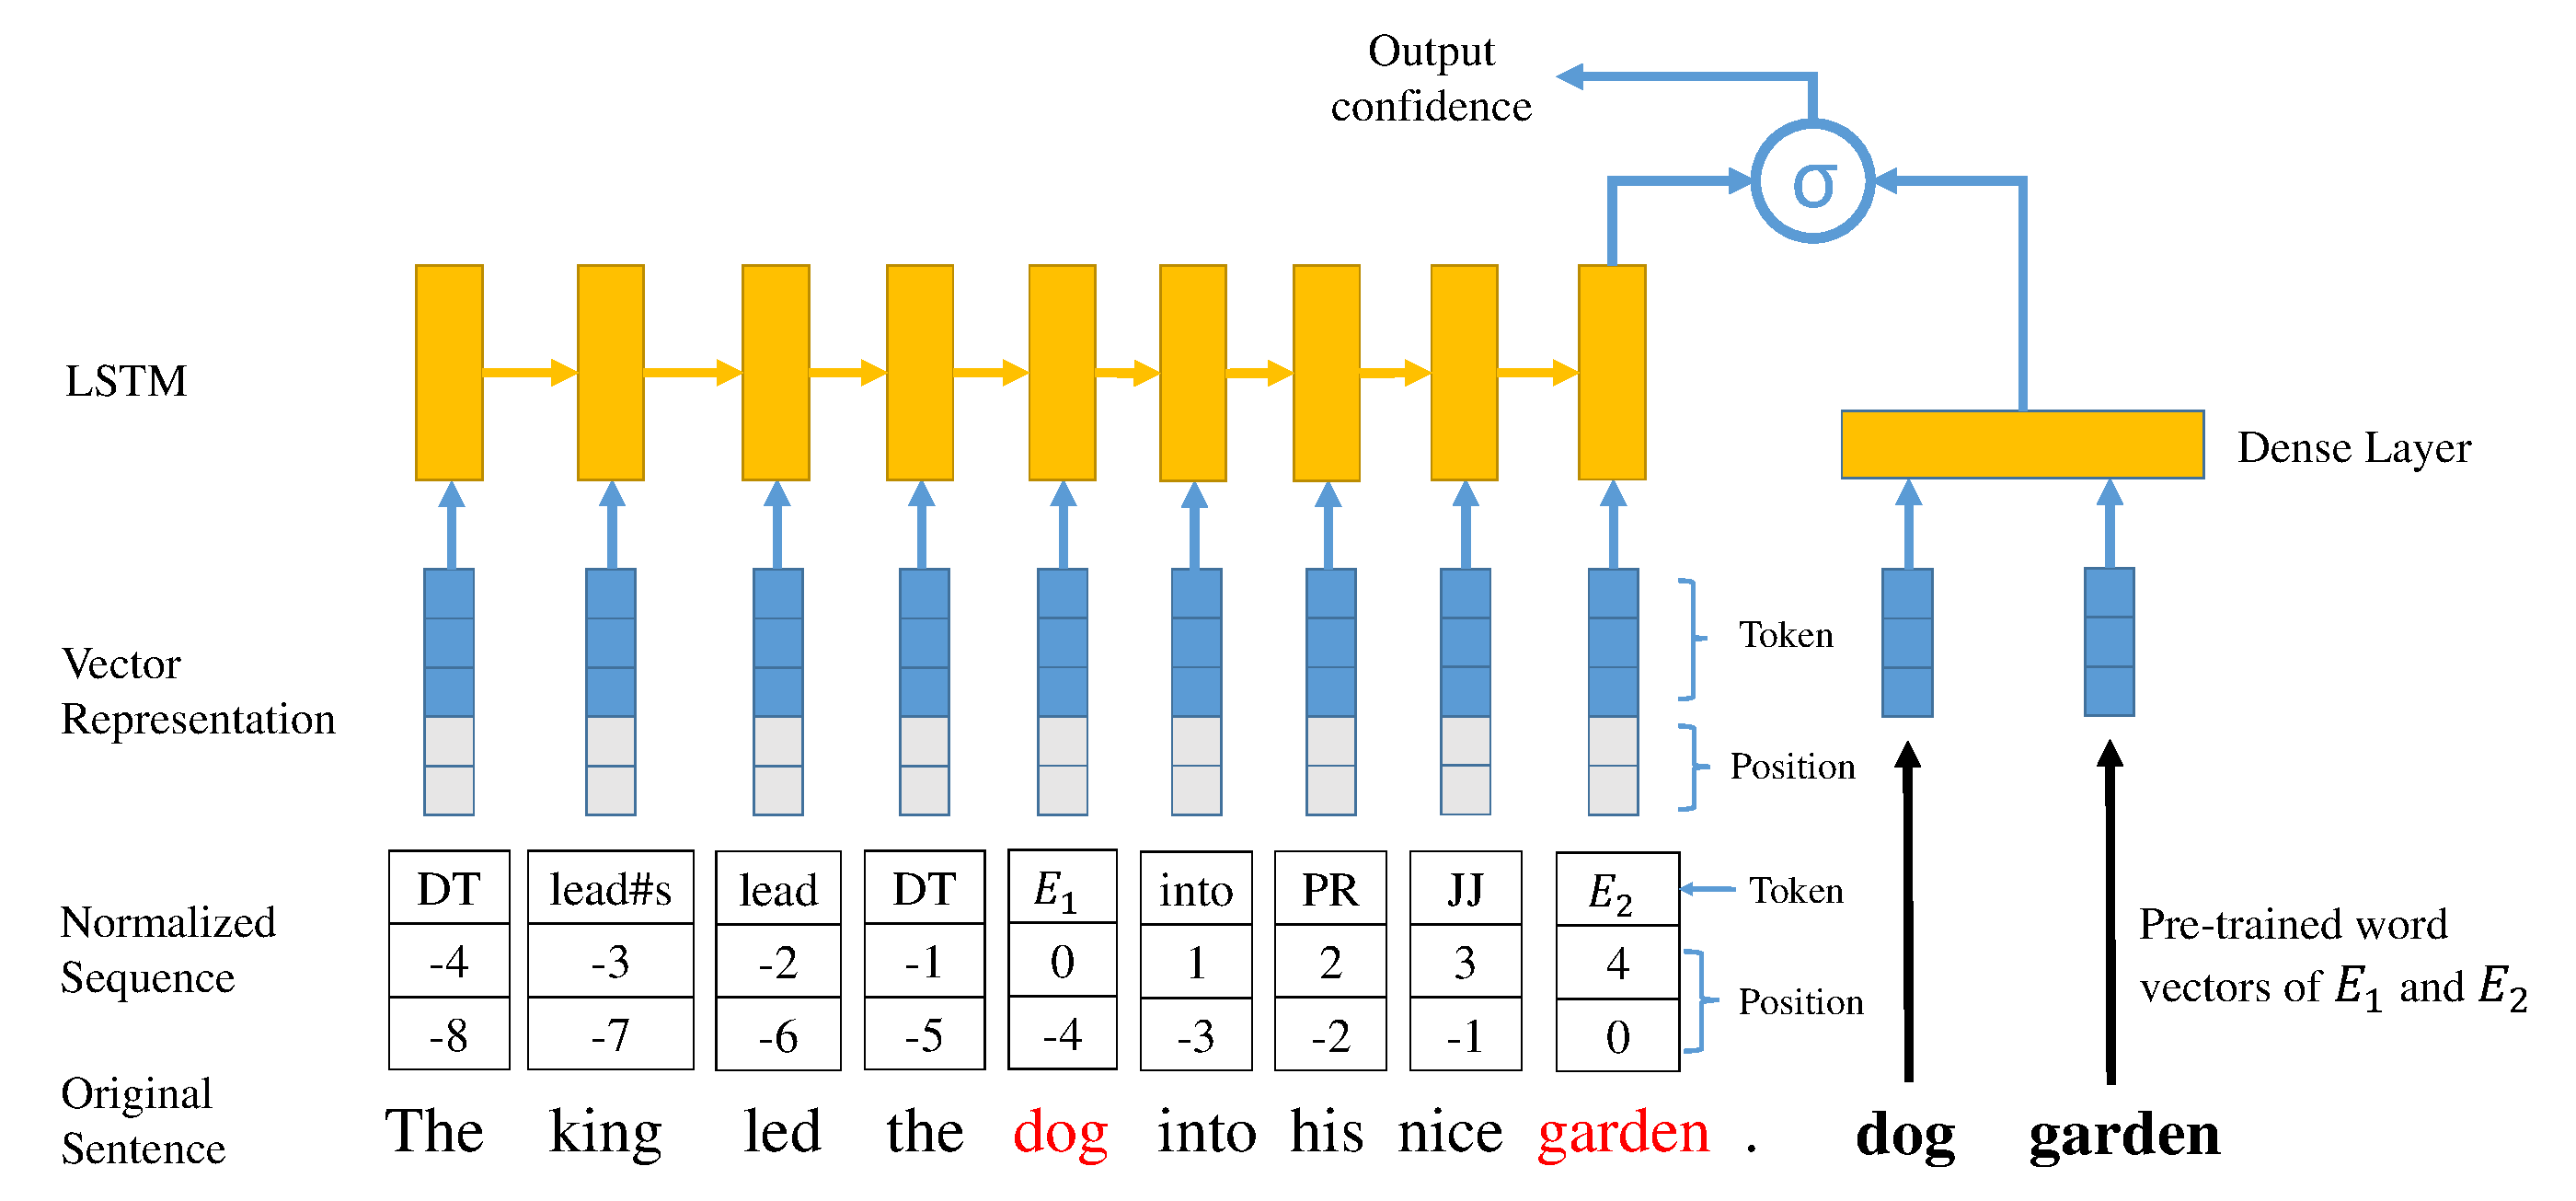
\epsfig{file=LSTM.pdf, width=0.8\textwidth}
	\caption{Our LSTM-based model}
	\label{fig:LSTM}
\end{figure*}

\noindent 
\textbf{Sentence Normalization}\\
We propose to use LSTM-based neural network for the first part to encode the sentence $s$.
As for the form of input sentences, 
if we use the original word sequence as the representation of a sentence $s$,  
it will cause three problems:

(i) The original word sequence concerns little syntactical information;
(ii) the irrelevant words in the sentence can take noise into model; 
(iii) the large vocabulary of original words induce too many parameters to tune in training process, which makes the network model unstable.

For example, given two sentences 
``\textit{The king led the dog into his nice garden.}'' and 
``\textit{A criminal led the dog into a poor garden.}''. 
The object pair is \textless \textit{dog, garden}\textgreater~for 
both sentences. The two words ``lead'' and ``into'', which are important
for determining whether the object pair is located near each other, are 
not given any more bias than the other words. 
Also, the semantic differences between irrelevant words, such as ``king'' and ``criminal'', ``beautiful'' and ``poor'', are not useful to the co-location
relation between the ``dog'' and the ``garden'', and 
thus tends to act as noise in training a classifier.
%Additionally, if our vocabulary size 

\begin{table}[th]
	\centering
	\small
	\begin{tabular}{l|l}
		\hline
		\textbf{Level}	&  \textbf{Examples}\\ 		\hline
		Objects	& $\textnormal{E}_1$, $\textnormal{E}_2$ \\ 		\hline
		Lemma & open, lead, into, ...\\ \hline 
		Dependency Role	& open\#s, open\#o, into\#o, ... \\ 		\hline 
		POS Tag	& DT, PR, CC, JJ, ... \\ 		\hline 
	\end{tabular}
	\caption{Examples of four types of tokens during sentence normalization. (\#s represents the subject of given verb or preposition, and \#o represents the object)}
	\label{tab:norm}
\end{table}

Considering such problems, we can use POS (part-of-speech) tags instead to capture a little more syntactical information and reduce the vocabulary size. 
However, this method loses too much semantic dependency between the words. 
We then propose a normalized sentence representation merging the three most important and relevant kinds of information about an instance: lemma, POS tag and dependency role. 
We first replace the two nouns for the object pair as $\textnormal{E}_1$ and $\textnormal{E}_2$, keep the lemmatized form of the original words for all the verbs, adverbs and prepositions, which are highly relevant to describing physical scenes. 
We replace the subjects and direct objects of the \textit{verbs and prepositions} with special tokens indicating their dependency roles. 
For the remaining words, we just use their POS tags. 
The four kinds of tokens are illustrated in ~\tabref{tab:norm}.
\tabref{tab:norm_eg} is an example of our normalized sentence representation. The object pair is \textless \textit{dog, garden}\textgreater.

\begin{table*}[!th]
\centering
\begin{tabular}{lllllllllllll}
		\hline
\textit{The }&\textit{king }&\textit{opened }&\textit{the}&\textit{door}&\textit{and}& \textit{led}& \textit{the}& \textit{dog }& \textit{into }& \textit{his }& \textit{nice }& \textit{garden.}\\		 
DT & open\#s & open & DT & open\#o & CC& lead& DT &$\textnormal{E}_1$ & into & PR & JJ& $\textnormal{E}_2$.\\	 \hline
\end{tabular}
\caption{Sentence Normalization Example}
\label{tab:norm_eg}
\end{table*}

\noindent \textbf{Model Description}
\\
We propose a neural network model as a classifier illustrated by ~\figref{fig:LSTM}.
At the bottom of the figure shows the original sentence, which is transformed to normalized sequence described above.
Apart from the normalized tokens of the original sequence, to capture more structural information, we also encode the distance from each token to $\textnormal E_1$ and $\textnormal E_2$.
Such \textit{word position embeddings} (position/distance features) are proposed by~\citeauthor{zeng2014relation} with the intuition that information needed to determine the relation between two target nouns normally comes from words which are close to the target nouns. We adopt this feature because it can help LSTM keep track of the position of $\textnormal E_1$ and $\textnormal E_2$, better knowing \textit{where} the two object words are.

Obtaining such representation, we leverage a long-short-term-memory (LSTM) based neural network to encode the whole sequence of the tokens of our normalized representation. On the other hand, two pre-trained word vectors of the original two physical objects words are fed into a hidden dense layer. 
Then, we concatenate the encoded LSTM cell outputs with the dense hidden layer outputs.
Finally, we use \texttt{sigmoid} activation function to get the 
probability output of the input instance having the co-location relation 
between the two given objects. For hyperparameters selection and tuning, refer to experiments for our results.

\noindent \textbf{Training Objective \& Optimizer}\\
We choose to use the widely-used standard binary cross-entropy as our loss function.
The optimizer we choose is called RMSProp, which is an adaptive learning rate method proposed by by~\citeauthor{hinton2012neural}, suitable for recurrent neural networks.\\
\noindent
\textbf{Regularization}\\
A good regularization approach is needed to alleviate overfitting. Originally the conventional dropout methods proposed by \citeauthor{hinton2012improving} does not work well with recurrent neural networks with LSTM units, since dropout may hurt the valuable memorization ability of memory units. Following~\citeauthor{zaremba2014recurrent}, dropout in LSTM has been very successful by not only randomly dropping units for the inputs as well as the recurrent state update during training. Thus we use both types of the dropout methods to our LSTM model for it can obtain less interdependent network units and achieve better performance.

Another kind of regularization approach is batch normalization, proposed by~\citeauthor{ioffe2015batch,cooijmans2016recurrent}. It is used to solve the internal covariate shift problems as it make the network adapt to such shift, resulting slower convergence. As a result, it provides faster convergence and performance is said to be as good as (if not better than) unnormalized LSTM. 

%The intuition behind our model is that we 
\subsection{Extraction of \lnear\ Relation}
\label{sec:mine}
%Figure x shows the overall workflow of our automatic framework to mine LocatedNear relations from raw text.
%We first construct a vocabulary of physical objects. 
%
%For each sentence in the corpus, if a pair of physical objects
%$e_i$ and $e_j$ appear as nouns in the sentence, then we apply a LocatedNear relation classifier on the sentence as well as the object pair. 
%The classifier yields a probabilistic score $s$
%that indicates whether the pair has a LocatedNear relation in this sentence.
%Finally, all such ($s$,$e_i$, $e_j$) triples are aggregated by the object pairs, where each
%pair is associated with a final score. 
%
%This forms the LocatedNear knowledge that we want to acquire.

\figref{fig:overview} shows the overall workflow of our framework of
automatic extraction of \lnear\ relationship from text. 
For each object pair in the $n$ object pairs, say \textless$e_i,e_j$\textgreater , 
we find all the $m$ sentences in our corpus mentioning both objects. 
Then, we classify these $m$ instances with the object
co-location classifier and get the output confidences, which we regard as input into a function $f$ to obtain the final score of the object pair for their \lnear\ relation. After scoring each pair, we can set a threshold to extract the new instances of \lnear\ relation.
We propose five baseline $f$ functions as follows:
\begin{align*}
	f_0 &= m\\
	f_1&=\sum_{k=1}^{m} \textnormal{conf}(s_k,e_i,e_j) &f_2&=\frac{1}{m}\sum_{k=1}^{m} \textnormal{conf}(s_k,e_i,e_j)\\
	f_3&=\sum_{k=1}^{m}
	1_{ \{ \textnormal{conf}(s_k,e_i,e_j)>0.5 \} } 
	&f_4&=\frac{1}{m}\sum_{k=1}^{m} 
	1_{ \{ \textnormal{conf}(s_k,e_i,e_j)>0.5 \} }
\end{align*}

\begin{figure*}[th]
	\centering
	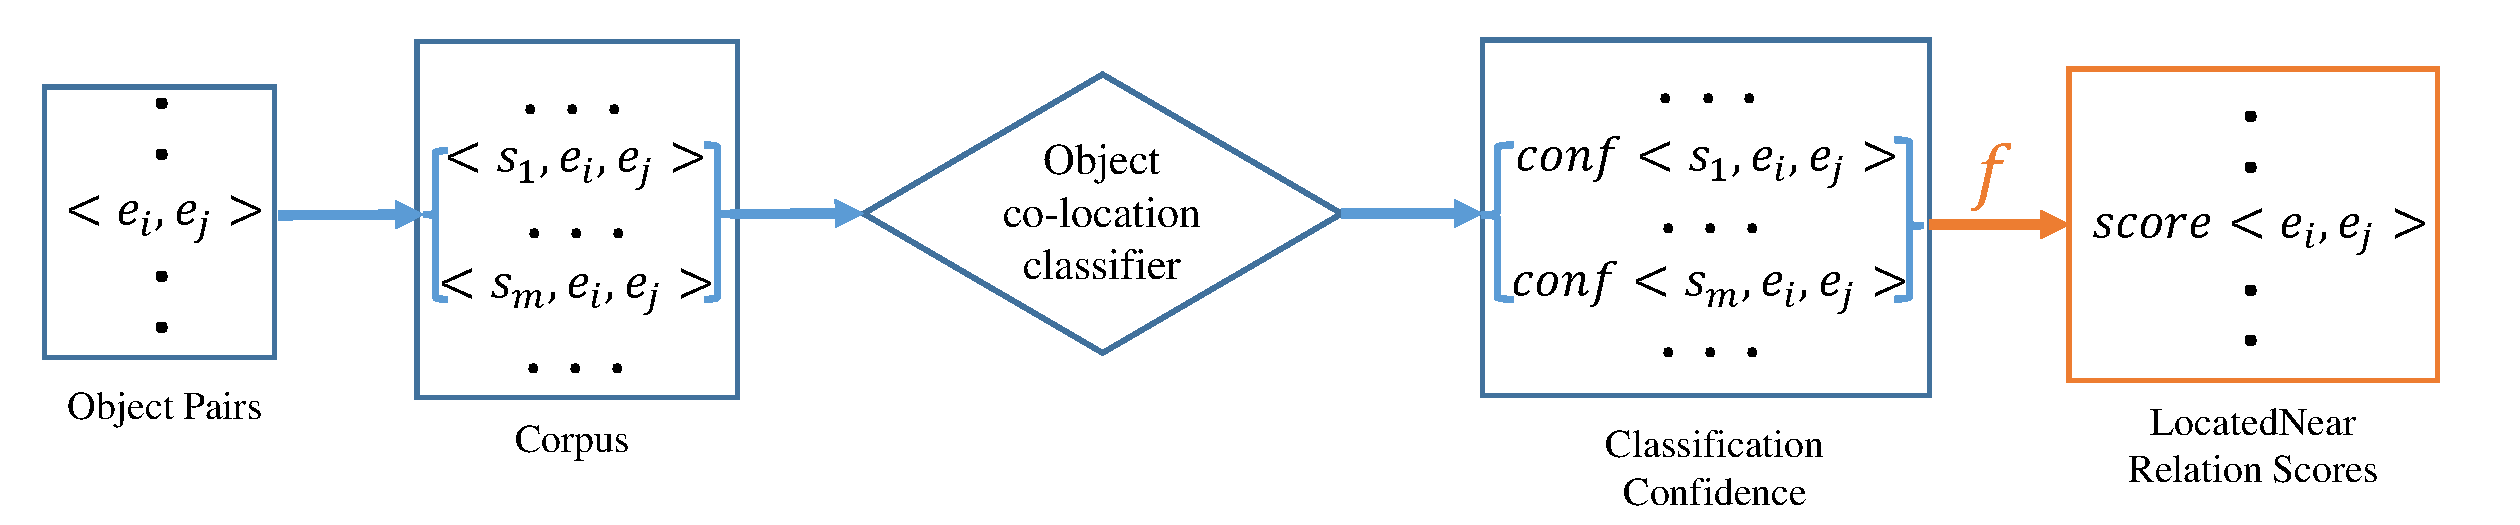
\epsfig{file=overflow.pdf, width=0.9\textwidth}
	\caption{Computing the \lnear\ scores of object pairs}
	\label{fig:overview}
\end{figure*}
$f_0$ is the simplest approach that returns the number of sentences
that contains the object pair,
$f_1$ is the sum of the confidence of all the $m$ instances, $f_2$ is the average of the $m$ confidence scores, 
$f_3$ is the number of the sentences whose confidence is higher than 0.5, 
and $f_4$ is the ratio between the number of the sentences whose confidence is higher than 0.5 and $m$.

